\chapter{How to Take Charge of Your Life}

This chapter follows an original Jim Rohn lecture preserved in a curated playlist rather than a clean institutional course. We keep the local order of the talk because the lecture derives its force from sequence: first a governing rule, then a marketplace puzzle, then a model of seasons, then a pair of practical laws, and only after that the long implementation block on goals, asking, and decisive action. Where the transcript briefly garbles, we retain only what the surrounding argument securely establishes. Curation credit for the playlist belongs to LazyingArt LLC.

\section{Opening Challenge and Seminar Frame}

\begin{figure}[t]
\centering

\includegraphics[width=.78\linewidth]{lecture_16_figure_01.png}
\caption{Opening seminar frame. The chalkboard heading is visibly \emph{Personal Dev.}; the fuller phrase \emph{Personal Development} is supported by the spoken context rather than fully legible chalk.}
\end{figure}

The board does not give us a worked derivation. It gives us a title and a setting, and that is enough. The visible chalk supports only the abbreviated heading \emph{Personal Dev.}; the lecture itself supplies the fuller sense. Before we are allowed to discuss method, goals, or attitude, the talk fixes a governing relation:

\begin{align}
\text{Have More} &\Longleftarrow \text{Become More},\\
\neg(\text{change in self}) &\Longrightarrow \text{same outcomes}.
\end{align}

Rohn immediately adds a companion verbal inequality which is better kept in words than forced into a heavier symbol:

\begin{equation}
\text{Income does not far exceed personal development.}
\end{equation}

The claim is structural, not econometric. Lucky jumps occur, but they do not hold unless the person grows to the level of the jump. That is why the lecture's million-dollar example is not a joke. If somebody hands us a million dollars, we had better become a millionaire quickly enough to keep it.

This early cluster of remarks is not only about money. The same rule is immediately extended to success and happiness. Success is something we attract rather than merely pursue. The major question on the job is not simply what we are getting; it is what we are becoming there. True happiness is not contained in what we get, but in what we become. Hence personal development is not one topic among many. It is the lecture's hidden variable.

Rohn even pauses to say that of all the assignments Mr. Shoaff gave him at age twenty-five, this one was probably the most difficult, and that he is still working on it. That remark matters. It prevents the chapter from sounding like a closed theorem. The lecture is presenting a rule, but it is also presenting a lifelong task.

Only after that does he preview the evening's later subjects: basic laws, goal-setting, diseases of attitude, and the emotions that can turn a life around in a day. This preview should remain in the chapter because it preserves the seminar rhythm. But the lecture soon reconverges on the sentence that governs the whole evening:

\begin{equation}
\text{The major key to your better future is you.}
\end{equation}

\begin{figure}[t]
\centering
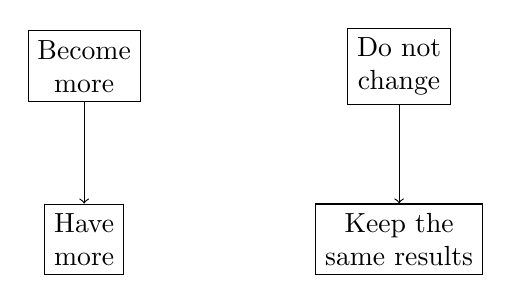
\begin{tikzpicture}[x=1cm,y=1cm]
\node[draw, align=center] (a) at (-2,2.2) {Become\\more};
\node[draw, align=center] (b) at (-2,0.0) {Have\\more};
\node[draw, align=center] (c) at (2,2.2) {Do not\\change};
\node[draw, align=center] (d) at (2,0.0) {Keep the\\same results};
\draw[->] (a) -- (b);
\draw[->] (c) -- (d);
\end{tikzpicture}
\caption{Transcript-based opening schema. The lecture begins with a directional rule about the self, not with a forecast about the world.}
\end{figure}

\section{Value, Compensation, and Self-Work}

With the theme fixed, the lecture raises its first serious puzzle. Two people work for the same company, in the same community, with the same products, the same traffic, the same problems, yet one makes a thousand a month and the other makes two thousand. Rohn insists on the long sameness of the list because he wants the eventual answer to do real explanatory work.

\subsection{Question \& Answer}

\paragraph{Question.} Why do two apparently similar people get very different economic results?

\paragraph{Answer.} Not because one possesses more hours in the day, but because one brings more value to the marketplace in the same time.

To keep the logic visible, let us introduce only the lightest notation. Let \(T\) denote the fixed time available in a period, let \(V\) denote value brought to the marketplace, and let \(I\) denote income or compensation. Then the lecture's practical claim can be written as

\begin{align}
I &\propto V,\\
I &\neq \text{time alone}.
\end{align}

The rhetorical middle step matters and should not be skipped. Rohn first tries the wrong variable. Perhaps, he says, time makes the difference. But then he breaks the thought immediately: there is no extra time. We cannot borrow Harold's hours, and when the clock strikes midnight the day is finished. Once time is ruled out as the adjustable variable, value enters not as a slogan but as the only serious candidate left.

That leads to the lecture's worked economic example:

\begin{align}
I_1 &= kV_1, \qquad I_2 = kV_2, \qquad T_1=T_2,\\
V_2 &= 2V_1 \Longrightarrow I_2 = 2I_1,\\
V_2 &= 3V_1 \Longrightarrow I_2 = 3I_1.
\end{align}

Thus the local derivation is simple: hold \(T\) fixed, raise \(V\), and the result can rise without any appeal to extra hours. This is exactly the tension Rohn wants to preserve when he asks whether it is possible to become twice as valuable and make twice as much money in the same time. His answer is yes, if one goes to work primarily on oneself.

That is why the lecture immediately widens again from value to character. Above-average income follows from becoming an above-average person. The examples are concrete on purpose: handshake, smile, excitement, interest in other people, intensity to win. They are not stray bits of motivational fluff. They are local, human-scale instances of the same law. If we want above-average results, we must become a more capable causal instrument.

This also explains one of the lecture's most quoted maxims, which belongs at the end of the block because it is the compensation argument recast as a rule for conduct: learn to work harder on yourself than you do on your job. Without that sentence, the mathematics of value would remain detached from the speaker's intended application.

\section{Seasons, Change, and the Four Major Lessons}

After the marketplace puzzle is solved, the lecture blocks an easy escape. We are not permitted to say that perhaps the next decade, or the next employer, or the next turn in public conditions will finally stabilize things for us. Rohn's answer about the eighties is devastating because it is so plain: they will be about like it has always been.

This is then unfolded through recurring structures: tide in and tide out, light and dark, fall and winter. The point is not novelty. The point is regularity. External conditions rotate. Some winters are long, some are short, some hard, some easy, but winter itself is not up for negotiation. The world, as the lecture reads it, offers opportunity mixed with difficulty.

\subsection{Question \& Answer}

\paragraph{Question.} If life is not going to change, how can my life change?

\paragraph{Answer.} When we change. The only way it gets better for us is when we get better.

Rohn compresses the turn into two phrases:

\begin{align}
\text{Life and business} &\sim \text{the changing seasons},\\
\text{You cannot change the seasons} &\Longrightarrow \text{change yourself instead.}
\end{align}

And then he adds the decisive gloss: life gets better not by chance, but by change.

The lecture's seasonal scaffold may therefore be written as

\begin{equation}
\text{Winter} \to \text{Spring} \to \text{Summer} \to \text{Fall} \to \text{Winter}.
\end{equation}

\begin{figure}[t]
\centering
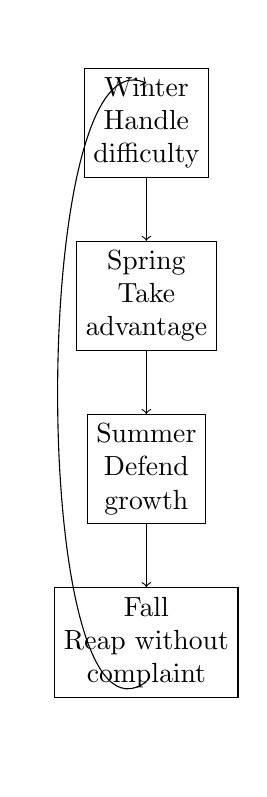
\begin{tikzpicture}[x=1cm,y=1cm]
\node[draw, align=center] (w) at (0,6.0) {Winter\\Handle\\difficulty};
\node[draw, align=center] (s) at (0,3.8) {Spring\\Take\\advantage};
\node[draw, align=center] (u) at (0,1.6) {Summer\\Defend\\growth};
\node[draw, align=center] (f) at (0,-0.6) {Fall\\Reap without\\complaint};
\draw[->] (w) -- (s);
\draw[->] (s) -- (u);
\draw[->] (u) -- (f);
\draw[->] (0,-1.1) .. controls (-1.5,-2.2) and (-1.5,7.2) .. (0,6.5);
\end{tikzpicture}
\caption{Transcript-based seasonal scaffold. The lecture attaches one practical task to each season and then repeats the cycle.}
\end{figure}

The four lessons are then unfolded in order.

\begin{enumerate}
\item Learn how to handle the winters. Winter stands for difficulty, recession, heartbreak, confusion, and the periods in which things do not work. We cannot tear January off the calendar. We can, however, get stronger, wiser, and better. This is where the lecture places one of its most useful slogans: do not wish it were easier; wish you were better.

\item Learn how to take advantage of the spring. Spring is opportunity. It follows winter with regularity, but regularity alone does not help us unless we act. The lecture insists on the phrase \emph{take advantage}. Opportunity is real, but it is not self-harvesting. One either plants in the spring or begs in the fall. One must also act quickly, because the lecture repeatedly reminds us that only a handful of springs are handed to any one of us.

\item Learn how to protect the crops all summer. Summer is the time when what has been started is attacked. Bugs, weeds, intruders, and erosion are the lecture's symbols for a universal fact: beginnings do not defend themselves.

\item Learn how to reap in the fall without complaint. Fall is the reckoning. If the crop is good, reap without apology. If the crop is poor, reap without complaint. This is the first point at which the seasonal analogy is converted directly into an ethic of maturity.
\end{enumerate}

The two compact formulas that govern the summer lesson are among the lecture's clearest axioms:

\begin{align}
\text{All good will be attacked},\\
\text{All values must be defended}.
\end{align}

At this stage the lecture is still architectural rather than psychological. It builds a world in which difficulty and opportunity alternate, growth is vulnerable, and harvest cannot be argued away.

\section{Responsibility, Response, and the Setup of Life}

The move from seasons to personal agency happens through the long blame-list anecdote. Government, taxes, prices, weather, traffic, company policy, training program, relatives, neighbors, economy, community: Rohn lets the list become exhaustive so that its defect may later appear in full light.

\begin{remark}
The transcript is briefly corrupted at the precise moment when the list is torn up and replaced by the word \emph{me}, but the argumentative turn is unmistakable. The missing causal term is the self.
\end{remark}

\subsection{Question \& Answer}

\paragraph{Question.} What determines the quality and quantity of life?

\paragraph{Answer.} Not what happens, because what happens is broadly shared. The decisive term is what we do.

The lecture's operational rule can therefore be set down as

\begin{equation}
\text{What happens} \approx \text{the same for many people}, \qquad \text{What you do}=\text{difference-maker}.
\end{equation}

This is not a denial that circumstances matter. It is a reordering of causes. Rain falls on both salesman and non-salesman; the difference lies in response. One stays home because the storm is an excuse. Another goes out because the storm is a market condition. The world does not split into two weathers. It splits into two interpretations and two actions.

This is why Rohn immediately asks the forward question: what are we going to do starting tomorrow that will make a difference? The lecture does not leave the response principle in general form. It pushes it into time. If nothing changes tomorrow, the next five years will look too much like the last five.

\begin{equation}
\neg(\text{new action tomorrow}) \Longrightarrow \text{the next five years resemble the last five}.
\end{equation}

He then adds the almost comic but crucial reminder: if we do not like our present address, we can change it. We are not trees.

From here the lecture asks what actual life change requires, and the answer is no longer a slogan.

\paragraph{Discipline.} Enthusiasm is not enough. We may be excited about lifting two hundred pounds until we arrive at the gym. Then the next virtue is needed. Rohn names it plainly: discipline. Small disciplines matter because they build both results and muscle. The local update rule is

\begin{equation}
\text{Little disciplines} \to \text{discipline muscle} \to \text{capacity for larger challenges}.
\end{equation}

\paragraph{Self-motivation.} Others may influence us, but they cannot finally do our changing for us. Good people are not manufactured by force. They change themselves. That is why self-motivation cannot be outsourced.

\paragraph{Study.} The first step toward change is to find out how things work. Here the lecture becomes almost epistemological. Lack of money is not yet the deepest problem; lack of ideas is. Therefore the instruction is to study, to keep a journal, to repeat what works, and to read broadly enough that an idea may take root and later appear in bank account, dress, personality, and lifestyle.

\paragraph{Curiosity.} Rohn sharpens the mood of study by calling for childish curiosity. The child asks until the thing is known. The adult too often stops at convenience. This is why reading occupies so much space in the lecture: it is curiosity given a durable instrument.

Rohn then names the world as a structure governed by laws. We may not like the arrangement, but we had better learn it. The two reasons are exact and worth recording:

\begin{align}
\text{Learn the setup} &\Longrightarrow \text{avoid hurt},\\
\text{Learn the setup} &\Longrightarrow \text{benefit}.
\end{align}

This is why his examples become deliberately brutal. Do not walk out the tenth-story window. If a huge object keeps rising and crashing down in one place, the first intelligent move is to step out from under it. We do not need metaphysical agreement before practical alignment. We need the basic smartness to avoid being smashed.

\begin{figure}[t]
\centering
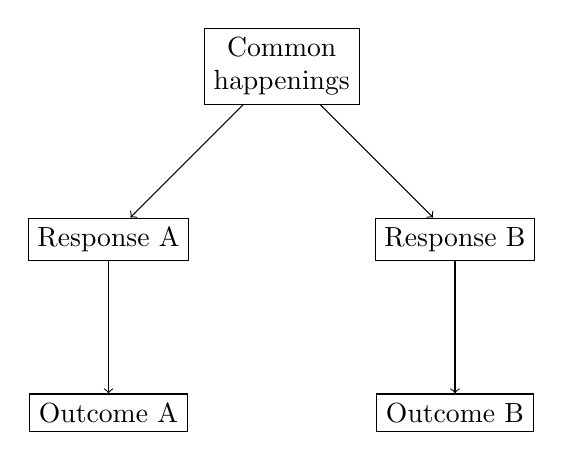
\begin{tikzpicture}[x=1cm,y=1cm]
\node[draw, align=center] (h) at (0,3.2) {Common\\happenings};
\node[draw, align=center] (r1) at (-2.2,1.0) {Response A};
\node[draw, align=center] (r2) at (2.2,1.0) {Response B};
\node[draw, align=center] (o1) at (-2.2,-1.2) {Outcome A};
\node[draw, align=center] (o2) at (2.2,-1.2) {Outcome B};
\draw[->] (h) -- (r1);
\draw[->] (h) -- (r2);
\draw[->] (r1) -- (o1);
\draw[->] (r2) -- (o2);
\end{tikzpicture}
\caption{Transcript-based response principle. The same event may branch into different outcomes because the decisive variable is response.}
\end{figure}

\section{Basic Laws: Use and Sowing/Reaping}

At this point the lecture is at its most axiom-like. The laws are biblical in source, but in the lecture they function as compact causal rules. This is the chapter's most explicit mathematical block, provided we remember that the mathematics here is schematic and practical rather than modern and technical.

\subsection{The Law of Use}

The first law is stated in a form so compressed that it already behaves like notation:

\begin{align}
\text{Whatever you do not use} &\Longrightarrow \text{you lose},\\
\text{Lack of use} &\Longrightarrow \text{loss}.
\end{align}

The arm tied to the body is the simplest example. Leave it unused long enough and use is forfeited. The point is then generalized across the human inventory.

\begin{table}[h]
\centering
\begin{tabular}{ll}
Arm & unused \(\Longrightarrow\) lost \\
Ambition & unused \(\Longrightarrow\) declines \\
Strong feeling & unused \(\Longrightarrow\) diminishes \\
Faith & unused \(\Longrightarrow\) decreases \\
Energy & unused \(\Longrightarrow\) decreases \\
Ability & unused \(\Longrightarrow\) lost
\end{tabular}
\caption{Compact statement of the law of use.}
\end{table}

The law is deliberately harsh because it is meant to remove sentimental thinking. Unused faculties do not wait politely for a future vote. They decline automatically. The practical corollary follows at once: take a new inventory of yourself. Make sure talent, ability, mentality, ingenuity, vitality, strong feeling, faith, and courage are being used. Otherwise they are not merely idle. They are being diminished.

The parable of the talents is then retold as an illustration of the same law. The servant who buries the talent is not condemned for reckless loss but for sterile preservation. What is merely kept safe is still, in the lecture's logic, forfeited if it is not employed.

\subsection{The Law of Sowing and Reaping}

The second law begins in its familiar forward form,

\begin{equation}
\text{Whatever you sow} \Longrightarrow \text{you reap},
\end{equation}

but the lecture's real explanatory turn comes when the formula is reversed:

\begin{equation}
\text{Whatever you reap}=\text{what you have sown}.
\end{equation}

This reversal locates cause. If the crop is disappointing, we do not first interrogate fate. We look for the planter. And the lecture's answer is precise enough to count as a derivation:

\begin{align}
\text{Disliked crop} &\Longrightarrow \text{find the planter},\\
\text{find the planter} &\Longrightarrow \text{look in the mirror}.
\end{align}

This is why the mirror arrives in the lecture exactly here. The blame-list is over. Cause has become personal again.

Rohn then begins to unpack the law. Its strongest displayed forms are

\begin{align}
\text{If you sow bad} &\Longrightarrow \text{reap bad},\\
\text{If you sow good} &\Longrightarrow \text{reap good},\\
\text{Reap} &\gg \text{Sow},\\
\neg(\text{sow}) &\Longrightarrow \neg(\text{reap}).
\end{align}

\begin{remark}
The numbered middle of the seven-point list is partially garbled in the transcript. The secure points are the negative case, the positive case, the amplification claim, the qualification that sometimes one loses anyway, and the final zero case: if one does not sow, one does not reap. The intermediate bridge is therefore reconstructed cautiously at the level of argument rather than verbatim wording.
\end{remark}

The seven-point structure can then be recorded as follows.

\begin{enumerate}
\item The law is negative: if we sow bad, we reap bad.
\item The law is positive: if we sow good, we reap good.
\item The law is amplifying: we do not merely reap what we sow; we reap more.
\item The multiplier works in both directions; on the negative side, sowing to the wind becomes reaping the whirlwind.
\item Plans compound through time. We are always buying some plan, chosen or drifted into, and time will carry that plan forward.
\item Sometimes we lose anyway. A good farmer may still lose the crop to hail. This is not a refutation of the law but a qualification of the planet.
\item If we do not sow, we do not reap. In that case we do not even give the law a chance to operate on our behalf.
\end{enumerate}

The lecture is careful here. Law does not eliminate contingency. The world may still hail on the crop and rain on the parade. But contingency is not permission for passivity. It is the reason to sow early, sow well, and stop confusing drift with innocence.

\section{Goals, Reasons, and the Art of Asking}

Only after the laws have been stated does the lecture turn fully to goals. This order matters. Goals are not presented as arbitrary wishing but as a way of cooperating with reality once reality has been studied.

Rohn frames the transition with one of the lecture's sharpest alternatives:

\begin{equation}
\text{Make a living} \quad \text{or} \quad \text{design a life.}
\end{equation}

The whole point of goals is to prevent existence from deteriorating into mere economic survival. The first principle of this block is then given in a sentence we should not dilute:

\begin{equation}
\text{Reasons come first; answers come second.}
\end{equation}

This is why the lecture spends so much time on reasons. The block on cookies, the money clip, debt collectors, family travel, Andrew Carnegie, and the friend who got mad enough to get rich is not ornamental. It is there to prove that reasons need not be lofty to be effective. They need to be vivid enough to move conduct. Wealth, in this lecture, is less a matter of bare intelligence than of sufficiently heated inspiration.

Goals are then divided in two ways.

\paragraph{By range.}
\begin{itemize}
\item Long-range goals: dreams for the next three, five, ten, twenty, or forty years.
\item Short-range goals: tomorrow, this week, this month, this year; these are confidence builders.
\end{itemize}

\paragraph{By category.}
\begin{itemize}
\item Economic goals.
\item Goals for things.
\item Personal-development goals.
\end{itemize}

The ordering is again deliberate. Economics matters and should be planned meticulously. Material things belong on the list as real objects of effort and celebration. But personal-development goals are the category that explains the other two, because the person who becomes more skillful attracts better conditions.

He then turns goal-setting into a three-step procedure.

\begin{enumerate}
\item Work on your goals.
\item Write your goals down.
\item Check the size and kind of your goals, because goals are affecting you all day long.
\end{enumerate}

This leads to the lecture's correction of passive wishing:

\begin{equation}
\text{Hope} \neq \text{Plan}.
\end{equation}

Everyone hopes. The future improves by plan.

From here the lecture compresses desire into a single imperative:

\begin{equation}
\text{Ask}.
\end{equation}

And then, in slightly expanded form,

\begin{equation}
\text{Ask} \Longrightarrow \text{Receive}.
\end{equation}

Again we should not over-formalize. The lecture does not claim a mechanical theorem in the modern sense. It offers three practical clarifications:

\begin{align}
\text{Asking} &= \text{the beginning of receiving},\\
\text{Receiving} &= \text{automatic},\\
\text{Supply} &\text{ is abundant.}
\end{align}

Thus the shortage lies less in the ocean than in the size of the vessel we bring to it. Some people go to the ocean with a teaspoon.

Rohn then gives two rules for asking. Ask with intelligence: be specific, descriptive, and clear. Ask with faith: plan like an adult and believe like a child. The lecture's local logic is therefore

\begin{align}
\text{Clear description} &\Longrightarrow \text{stronger direction},\\
\text{Faithful asking} &\Longrightarrow \text{greater motivational pull}.
\end{align}

One last beat must be preserved here because it is easy to lose in a polished rewrite. Goals do not merely organize the future. They alter the bearer in the present. Our goals affect handshake, attitude, personality, walk, talk, and dress. In that sense goal-setting is not only planning. It is self-formation in forward-looking form.

\section{The Day That Turns Life Around and the Diseases of Attitude}

Rohn announced this subject very early in the seminar, and now at last he reaches it. That delay matters. By the time we arrive here, the lecture has already built the structure of change. The emotional sequence is not the structure itself. It is the ignition system.

The lecture even gives a broad definition in advance: civilization is the intelligent management of human emotions. The four emotions are then named, and action is added as the operative completion:

\begin{equation}
\text{Disgust} \to \text{Decision} \to \text{Desire} \to \text{Resolve} \to \text{Action}.
\end{equation}

\begin{figure}[t]
\centering
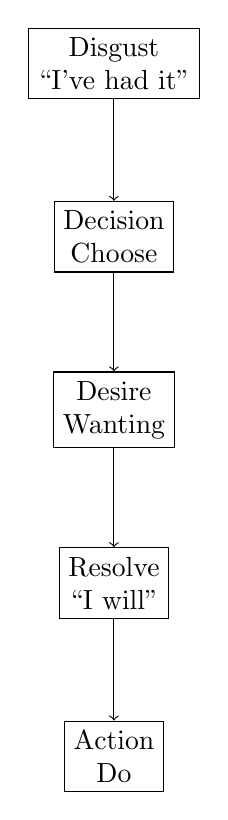
\begin{tikzpicture}[x=1cm,y=1cm]
\node[draw, align=center] (d1) at (0,8.0) {Disgust\\``I've had it''};
\node[draw, align=center] (d2) at (0,5.8) {Decision\\Choose};
\node[draw, align=center] (d3) at (0,3.6) {Desire\\Wanting};
\node[draw, align=center] (d4) at (0,1.4) {Resolve\\``I will''};
\node[draw, align=center] (d5) at (0,-0.8) {Action\\Do};
\draw[->] (d1) -- (d2);
\draw[->] (d2) -- (d3);
\draw[->] (d3) -- (d4);
\draw[->] (d4) -- (d5);
\end{tikzpicture}
\caption{Transcript-based emotional chain for the day that turns life around. The first four terms are emotions; the fifth is the activating completion.}
\end{figure}

Disgust is the moment at which one says, ``I have had it.'' The lecture returns to the broke-and-lying self at the door with the Girl Scout cookies because that scene gives disgust a precise psychological temperature. Decision follows: the inner civil war must be terminated by a choice. Desire is internal, though it may be triggered from outside by a book, sermon, lecture, conversation, or harsh event. Resolve is defined beautifully in the lecture as promising yourself you will never give up. And then action arrives as the trigger that converts feeling into results. The lecture's own final operator is practical: do something about how you feel.

But the seminar refuses to end with ignition alone. Every beginning can be attacked, and the final block names the counterforces.

\paragraph{Overcaution.} Life is all risky. If we think trying is risky, wait until we see the bill for not trying. Safety, pushed to the limit, becomes a corner under a sheet with three meals a day and no life in it.

\paragraph{Pessimism.} The pessimist lives by searching for what is wrong rather than what is right. This is why the half-empty and half-full glass matters in the lecture: not as a child's exercise in positivity, but as a statement that interpretation is itself causal. The same measure is given; the life is affected by how it is seen.

\paragraph{Poor thinking habits.} Here the lecture introduces another machine:

\begin{equation}
\text{As you think, so you become}.
\end{equation}

The mind is a factory. Thoughts, reading, and repeated inputs are ingredients. What goes in becomes the economic, social, and personal fabric of life. The lecture's point is sharp: poor thinking habits keep many people poor more reliably than poor working habits do.

\paragraph{Mental ingredients.} The high-school coffee example gives the lecture's most memorable image. Sugar and strychnine are both inputs, but not equivalent ones. The resulting rule is plain: watch your coffee. It does not matter who hands us the poison; poison still works. Therefore the practical imperative is to stand guard at the door of the mind.

\paragraph{Complaining.} The final disease is future-canceling murmuring. The Old Testament story of the children of Israel is used to make the point severe: complaining turns deliverance into desert. Spend five minutes complaining and five minutes are wasted; indulge long enough and the future itself is canceled.

By the end the tone has shifted from inspiration to vigilance. The war is on, mentally, personally, socially, and economically. One must not only begin well. One must defend what has been begun.

\section{Summary}

The lecture begins with a single governing relation and spends the rest of the evening unpacking it:

\begin{equation}
\text{A better future} \Longleftarrow \text{a changed self}.
\end{equation}

From that opening thesis everything else follows in order. The compensation puzzle replaces time with value. The seasons analogy blocks the fantasy that life will stabilize for us. The blame-list anecdote relocates cause in the self. Discipline, self-motivation, study, and curiosity turn agency into method. The law of use and the law of sowing and reaping provide the lecture's clearest causal structure. Goals, reasons, and asking convert law into program. Disgust, decision, desire, resolve, and action ignite the program. And the diseases of attitude remind us that beginnings are attackable and futures are cancelable.

What this chapter should preserve above all is not a bag of slogans but a progression. We are first told that becoming governs having. We are then shown, step by step, what a person would have to learn, ask, defend, and do if that opening sentence were taken seriously.